\documentclass{article}
\usepackage{pdfpages,fancyvrb}
\usepackage{siunitx}
\title{Petiteannonce package documentation}
\author{Vincent Bela\"\i che}
\begin{document}

\maketitle
\section{Introduction}
This is the documentation of the petiteannonce package. The aim of this package is to
make adverts that you would pin down on some notice board in a mall with your
phone number repeated on strips. This practice is quite common in France as it
is simple, cheap (no fee for intermediates like eBay\texttrademark),
and allows you to reach people in the same neighbourhood (so no need for
postal fee either).

\section{Package options}

There is one single class option \verb!margin!, this is used to set the margin value, by default this is
\SI{1}{\milli\metre}. For instance use:

\verb!\documentclass[margin=3mm]{petiteannonce}!

\noindent if you want it to be \SI{3}{\milli\metre} instead of \SI{1}{\milli\metre}.

\section{Commands}

There are three commands the \verb!\petiteannonce! command, the \verb!\petiteannoncewidth!
command, and the \verb!\petiteannonceaddtowidth! command.

\subsection{The \textbackslash petiteannonce command}

The \verb!\petiteannonce! command is used to create the advertisement. It takes two
mandatory arguments and one optional argument. 
\begin{itemize}
\item The 1\textsuperscript{st} mandatory argument is the phone number or
  email address where to reach the seller.
\item The 2\textsuperscript{nd} mandatory argument is the text of the advert itself
\item The optional argument is a list of comma separated \(<\textit
  key\/>=<\textit{value\/}>\) arguments that allows to configure a number of
  additional things. Absence of the key is equivalent to setting it to its
  default value. The supported keys are the following:
  \begin{list}{}{}
  \item [cols] positive integer with default value 1. Specifies the
    number of columns of the document that is used to compute the width of
    the advert. When the advert is repeated, a new paragraph is generated
    every {\em cols\/} columns.
  \item [count]  positive integer with default value 1. Tells the number of
    times the advert is repeated.
  \item [cutvspace] dimension with default value 10pt. Tell the vertical space
    under to horizontal dotted line that is provided for cutting one strip.
  \item [skip] non negative integer with default value 0. The value shall be
    less than {\em cols\/}. Specifies that the first {\em skip\/}
    advert are not generated. This may be useful when you want to make several
    adverts in the same document.
  \item [texthspace] dimension with default value 20pt. This key allows to
    specify the space evenly placed before and after advert text. 
  \item [textvspace] dimension with default value 10pt. This key allows to
    specify the space evenly placed above and below text.
  \item [telcolsep] dimension with default value 10pt. This key allows to
    specify the separation between two telephone strips, that is to say the
    horizontal space between the telephone numbers.
  \item [telrulewidth] dimension with default value 0.5pt. Width of the
    vertical rule separating two telephone strips.
  \item [telvspace] dimension with default value 10pt. Vertical space shared
    equally above and below the telephone number in the strip (this space is
    one the before and after the number if you look at the strip horizontally).
  \item [width] dimension with default value \verb!\textwidth!. Overloads the value
    computed with {\em cols\/}. In such a case take care to place the {\em
      width\/} argument after the {\em cols\/} argument. This specifies the advert total width, including the
    frame rule width, rule separator, and all the internal spaces.
  \end{list}
\end{itemize}

\subsection{The \textbackslash petiteannoncewidth and \textbackslash petiteannonceaddtowidth commands}

The \verb!\petiteannoncewidth! command takes one argument \#1 and expands into \#1 \(\times\) the width of the
advert text. This is useful when you use a tabular to make the text of the advert like in the example given in
\S~\ref{sec:sample-code}.

The \verb!\petiteannonceaddtowidth! command takes one argument that is some offset to add to the advert
textwidth. A use of that is given in example of \S~\ref{sec:sample-code}, where the advert text is within an
array, and one wants to take into account the \verb!\tabcolsep! half column separation.

\subsection{Changing the outside frame}

The frame around the advert is generated with a standard \verb!\framebox! command, so you can play with it by
changing \verb!\fboxsep! and \verb!\fboxrule!.

\section{Sample code}
\label{sec:sample-code}

The following sample code will expand into the advertisement page at the page
this sample code.


\VerbatimInput{petiteannonceexample.tex}



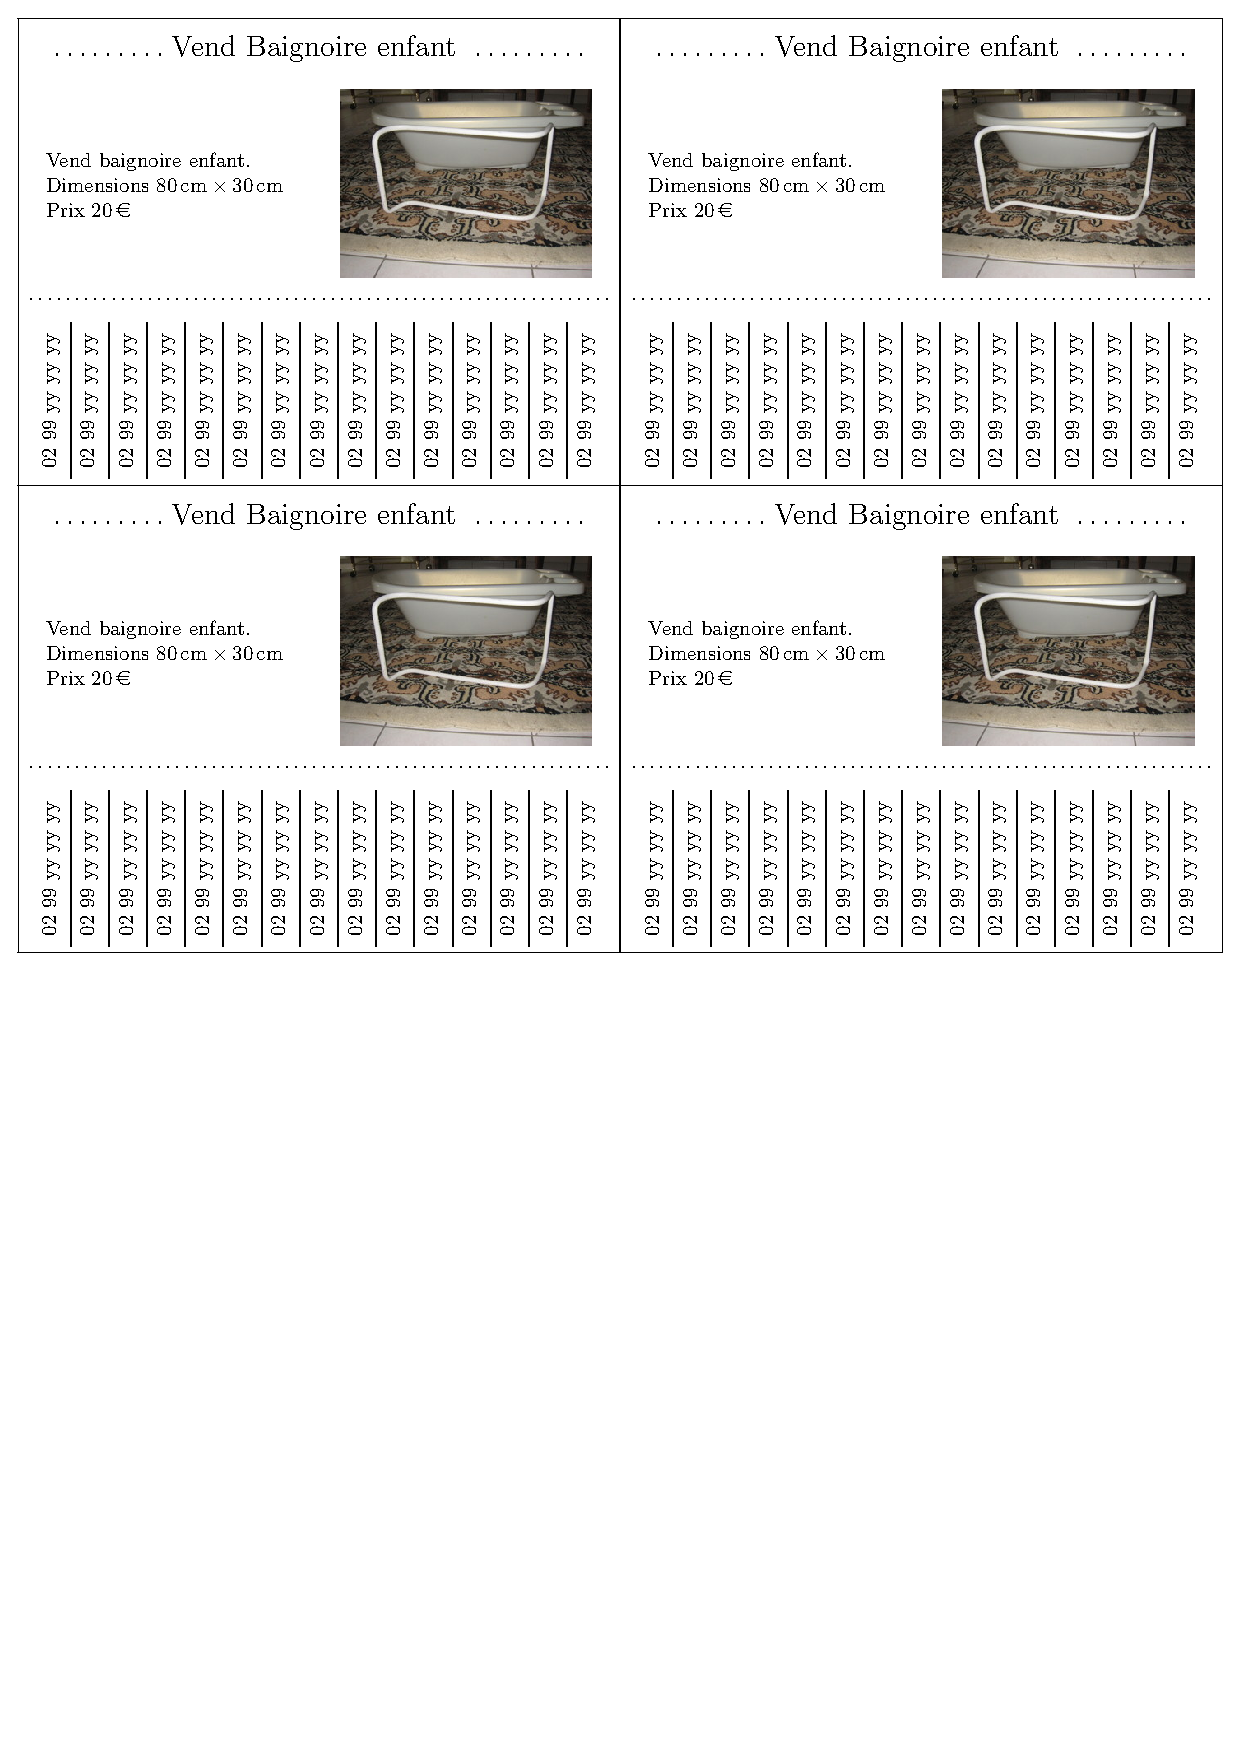
\includepdf{petiteannonceexample}

\end{document}

%%% Local Variables: 
%%% mode: latex
%%% TeX-PDF-mode: t
%%% TeX-master: t
%%% End: 
